\documentclass[11pt]{article}
%\usepackage{abbrevs}
\usepackage{natbib}
\usepackage{hyperref}
\usepackage{float}
\usepackage[pdftex]{graphicx}     % could insert ``draft'' between []
\pagestyle{empty}

\setlength{\oddsidemargin}{0pt} % there is 1 inch before the
                                % side margin in ``article'' class
\setlength{\textwidth}{6.5in}

\setlength{\voffset}{0pt}
%\setlength{\topmargin}{-36pt}     % there is 1 inch before the
\setlength{\topmargin}{-0.75in}     % there is 1 inch before the
                                % top margin in ``article'' class and
                                % then room for header, etc.
\setlength{\textheight}{10.0in}
%%%%%%%%%%%

\newcommand{\inch}{$^{\prime\prime}$}
\newcommand{\foot}{$^{\prime}$}

\begin{document}
\title{HERA Strawman Technical Design}
\maketitle
\begin{figure}[H]
\centering
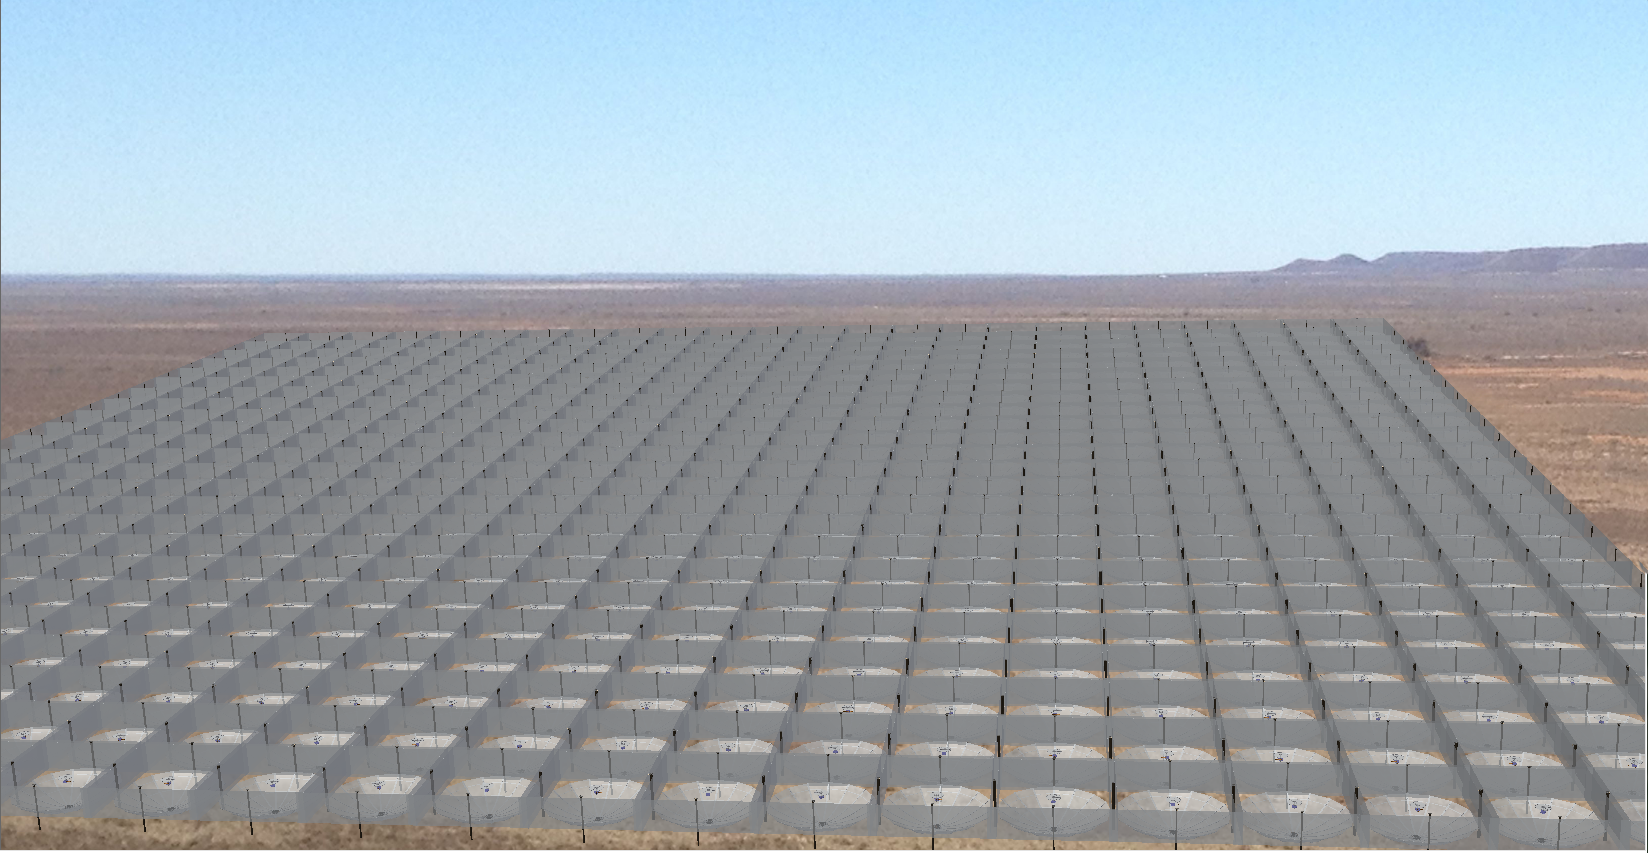
\includegraphics[width=\textwidth]{hera_14m_view0611-1252.png}
\end{figure}

\section{Introduction} 
This memo provides concise technical detail of a strawman design for HERA.  Although design iteration is certainly expected, given timelines for the current proposal round any major deviations should be known very soon.

To present a full design, this memo assumes specific values for parameters.  It will be pointed out what constraints and risks these impose for design iterations.  The following section will lay out those parameters, followed by descriptions of the major blocks of the telescope:

\begin{itemize}
\item Antenna
\item Front-end
\item Node
\item Correlator
\item Processor
\item Reticulation
\item Infrastructure
\end{itemize}

\section{Overall Configuration}
The specific values for high-level parameters are summarized in Table \ref{tab:overall}.

\begin{table}
\caption{Overall parameters and constraints.}
\label{tab:overall}
\begin{tabular}{|p{3cm}|p{3cm}|p{8cm}|}
\hline
{\bf Parameter} & {\bf Value} & {\bf Note} \\
\hline
N  &  576  & Roughly linear in cost (for N $<$ 1000 )and time, but low technical risk \\ \hline
Diameter & 14 m& Roughly (sub)-linear cost in area within about 8-15 m.  \\ \hline
Mount/optics & {\em f} 0.32 prime focus fixed-zenith with shield & $f/D$ can vary 0.3-0.4 with little impact. \\ \hline
Sampled frequency range & 0-250 MHz &  Sampling at 500 Msa/s.  Supported by electronics but need to investigate feed performance. \\ \hline
Processing bandwidth & 100 MHz & Many options of processing to yield sparse support at wide bandwidths along with a large EOR processed band.  Support F-engine at node. \\ \hline
Antennas per node & 16	 & Low risk. \\ \hline
Configuration	& 24 $\times$ 24 square grid & The strawman is heavily predicated on the regular square grid configuration but not the size.  Outliers are possible. \\ \hline
\end{tabular}
\end{table}

Figure \ref{fig:heraconfig576} shows the overall layout of antennas and distribution, which is obviously a regular square grid.  This allows tensioning of the elements against one another to minimize cost/performance.  Outliers are possible, but the per element cost will be higher.

\begin{figure}[H]
\centering
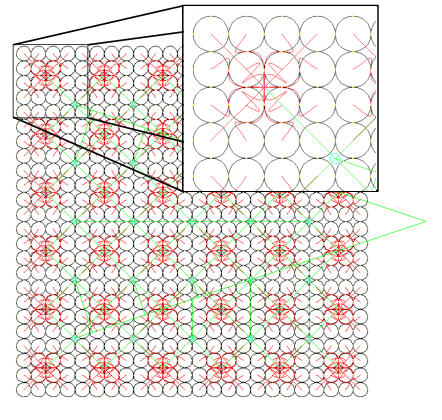
\includegraphics[width=12cm]{heraconfig576.png}
\caption{Overall layout of HERA.  Black circles are antennas, yellow circles are poles, red lines are antenna-node connections,  green is the shared signal/power trenches and cyan are power distribution points.  The square inset zooms in on one nodes worth - note that the red signal lines will be of equal length. }
\label{fig:heraconfig576}
\end{figure}

\section{Antenna}
The antenna is a 14-m fixed zenith faceted parabolic prime focus dish with an $f/D$ = 0.32.  The design principle is that a pipe loaded at the end can approximate a parabola.  Design parameters to be studied are pipe diameters (elasticity coefficients), launch angle and loading. Equations from
http://ruina.tam.cornell.edu/Courses/ME4735/Rand4770Vibrations/BeamFormulas.pdf
are shown in Figure \ref{fig:beam}.

\begin{figure}[H]
\centering
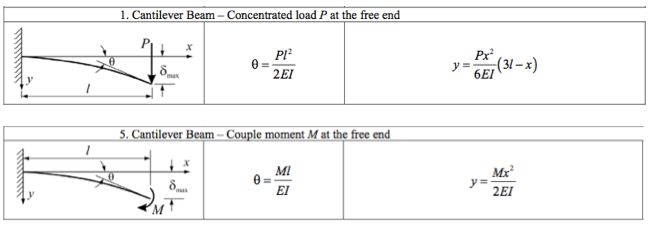
\includegraphics[width=\textwidth]{beam.png}
\caption{Shows equations for a loaded beam.}
\label{fig:beam}
\end{figure}

The focal ratio is set by the efficiency and the level of the standing wave ripple, which must be more than 60 dB down by the delays needed for the EOR detection.  Figure \ref{fig:heraDishfDplot} shows analytical calculations of the performance for antennas using a Gaussian feed matching the averages FWHM of the existing ''unflapped'' PAPER dipole and with 1.5m feed blockage.  A 10-meter and 12-meter antenna at about $f$=3.6 m are near the maximum efficiency of about 72\%.  The 10-meter antenna has a FWHM beamwidth of 13.4$^o$, the 12-meter FWHM=11.7$^o$ and the 14-meter ($f$=4.5) FWHM=9.8$^o$.  Calculated beampatterns are shown in Figure \ref{fig:HERA_10-12Beam}.  HFSS analysis of the full structures is being pursued and preliminary results are shown in Figure \ref{fig:pp}.

To reduce standing waves, one typically adds a ``splash cone'' directly below the feed to scatter the radiation.
If we posit that reflections must be suppressed by $-60$dB at delays corresponding to the time it takes
to travel 15m, and if we assume that reflections are attenuated by a factor $A$ for each crossing of the
attenuator placed below the feed, then the number of allowed reflections, $R$, is given by
\begin{equation}
R={\rm floor}\left(\frac{-60{\rm dB}}{2A}\right).
\end{equation}
Thus, for a feed height (or focal length), $f$, we have
\begin{equation}
2Rf<15{\rm m}.
\end{equation}
For a moderate attenuation value of $A=-15$dB, we have $f<4$m.

\begin{figure}[H]
\centering
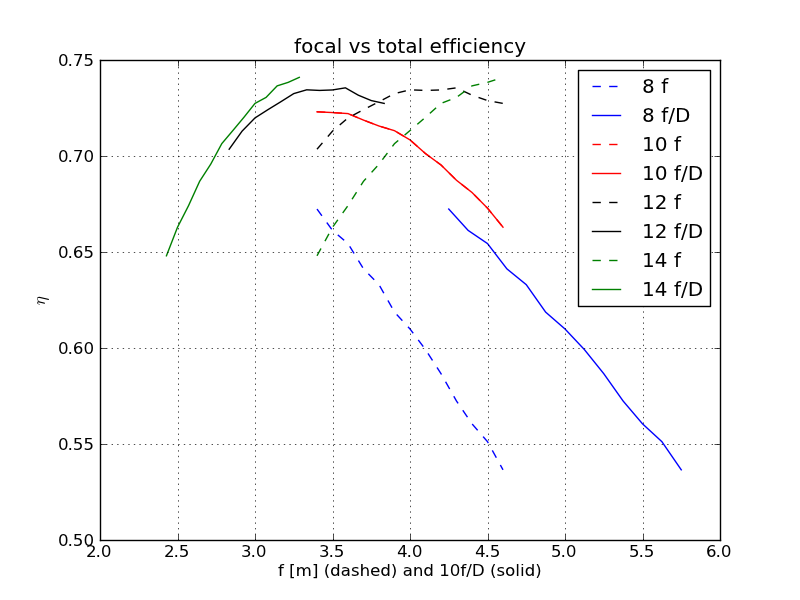
\includegraphics[width=\textwidth]{heraDishfDplot.png}
\caption{Antenna performance (overall efficiency) as a function of focal length and diameter, plotted two ways:  (1) versus focal length in m (dashed) and (2) versus 10$\times${\em f}/D (solid).  Note that the 10m curves are coincident (so the red line is both solid and dashed).}
\label{fig:heraDishfDplot}
\end{figure}

\begin{figure}[H]
\centering
\includegraphics[width=12cm]{hera_10-12-14Beam.png}
\caption{Analytical beam patterns for 10 and 12 meter antennas at $f$=3.6 and 14-meter at $f$=4.5.}
\label{fig:HERA_10-12Beam}
\end{figure}

\begin{figure}[H]
\centering
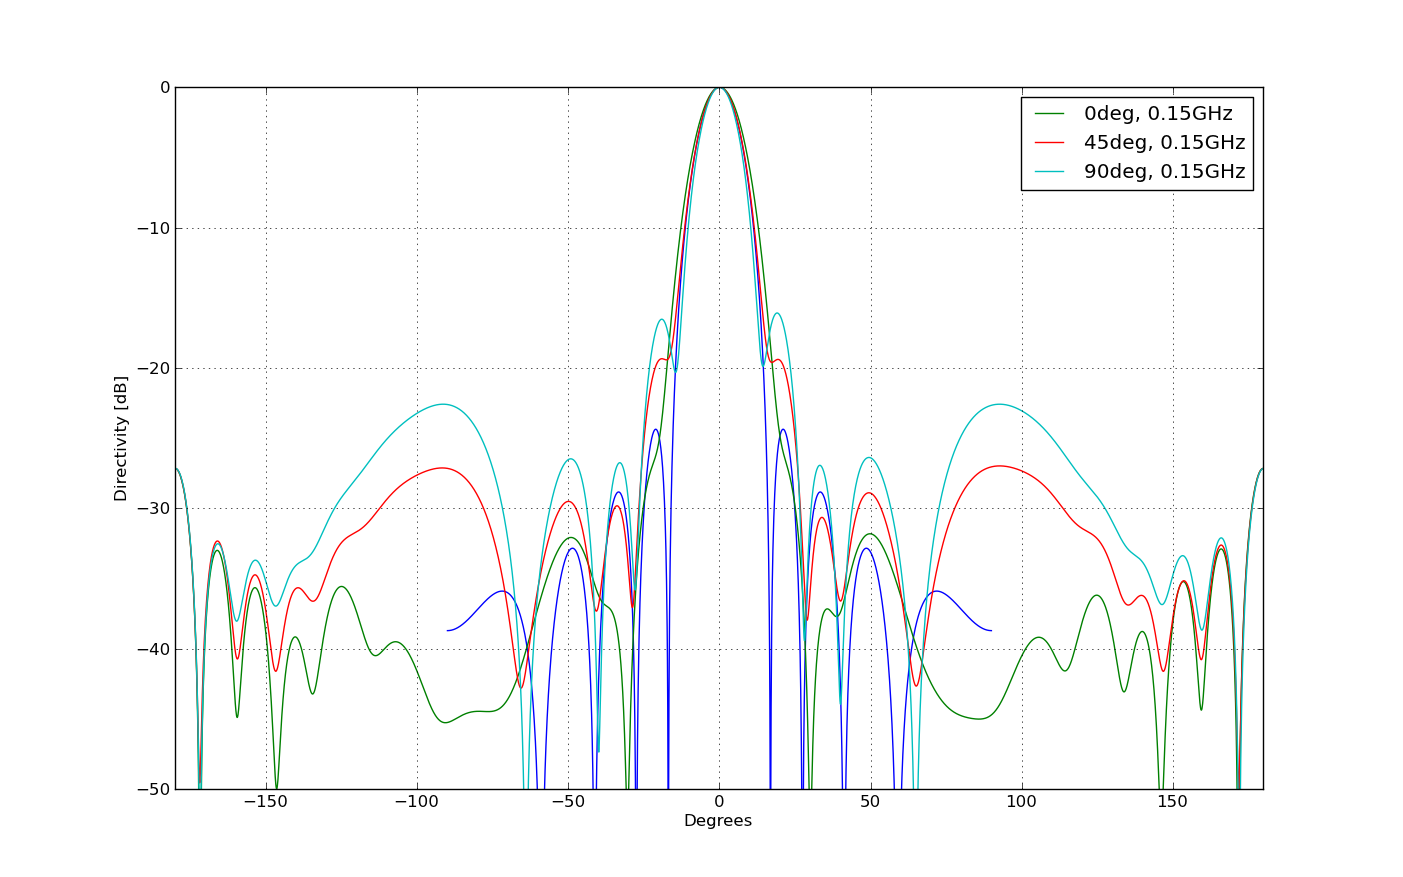
\includegraphics[width=12cm]{pp.png}
\caption{Preliminary HFSS beam patterns with analytical for 10-m antenna.}
\label{fig:pp}
\end{figure}

The overall accuracy in construction is contained within a few compact design features and transferred, primarily via the hub, PVC lengths and poles.  Accuracy is transferred from poles to hub to poles to stands.

The order of contruction (after trenching) is:
\begin{enumerate}
\item install poles to within $\pm$ 10 cm
\item survey poles and generate a best fit
\item install hubs
\item transfer height to poles, trim poles and install pole-tops
\item install feeds
\item transfer height to stands and install
\item install spars
\item install surface
\item conduct transformational science
\end{enumerate}

\subsection{Hub}
The central hub must be secure and sufficiently accurate.  The design is a concrete annulus holding pipes to launch the spars and supports.  Materials are concrete, sonotube and PVC pipe. The hub will also allow for the central feed tensioning line and a socket to install a ladder to access the feed.  It has a conduit out for signal and power.  Figure \ref{fig:hub} shows the engineering drawings.  The volume of concrete is about 4.4 ft$^3$ for a mass of about 600 pounds.
A jig will be used to make sure the sonotube are circular and concentric during the setup, pour and set of the concrete.

\begin{figure}[H]
\centering
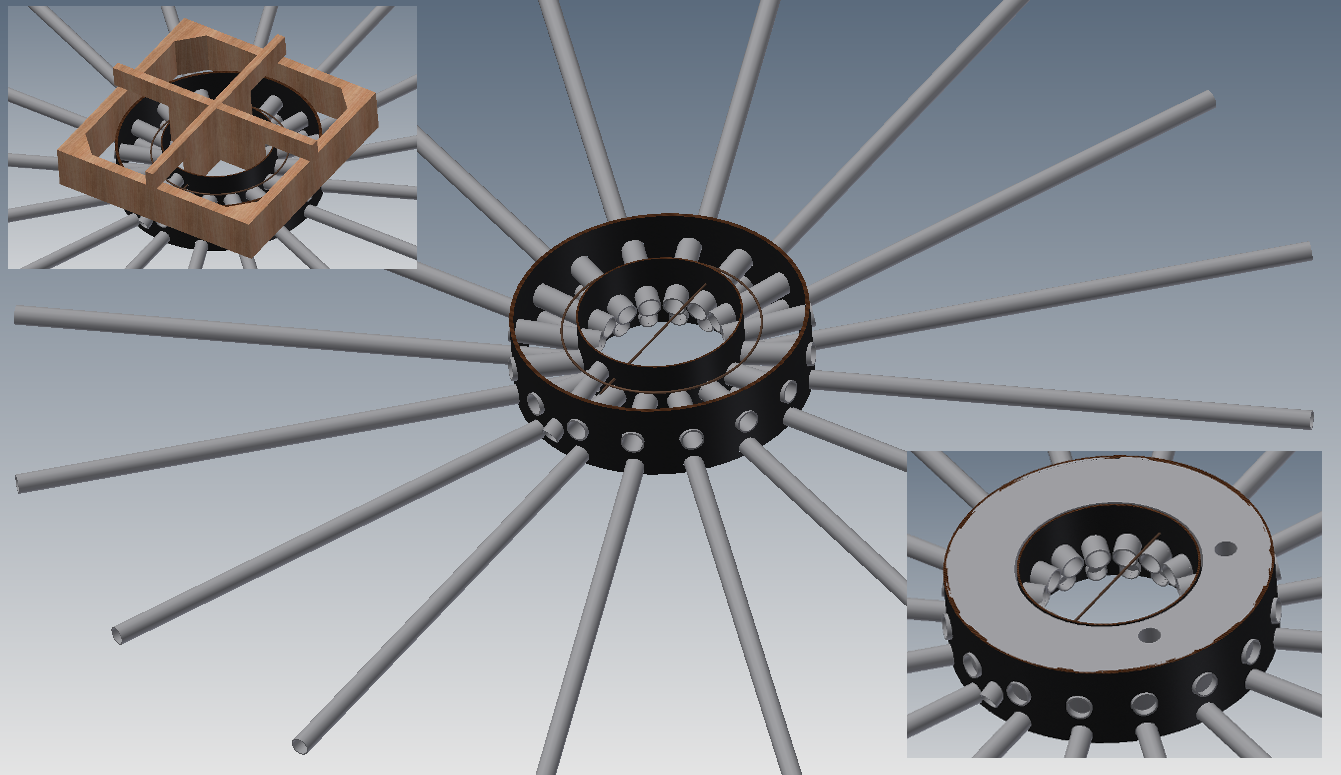
\includegraphics[width=\textwidth]{hub.png}
\caption{Center portion shows the hub without the concrete.  The upper left shows the support jig and the lower right has the completed hub.}
\label{fig:hub}
\end{figure}

The top set of PVC sleeves will hold the spars.  They are set at the optimal angle to generate the surface (to be determined by experiment - the angle of the parabola is $5^o$ at that point for a 36\inch{} diameter hub.  The bottom set of PVC position and anchor a ring of spar supports, discussed below.

\subsection{Spars}
The dish surface it set by sixteen spars emanating from the hub, which will be high-temperature (?) 2\inch{} PVC. 

The four quadrant spars will be firmly supported at the poles with fixtures, which will also position the circumferential support.  The fixtures will firmly hold the spar end at the correct angle for the parabolic shape.  

\subsection{Support}
The antenna support has the following members:  poles, stands and the inner ring, which are shown in Figure \ref{fig:support}.

\begin{figure}[H]
\centering
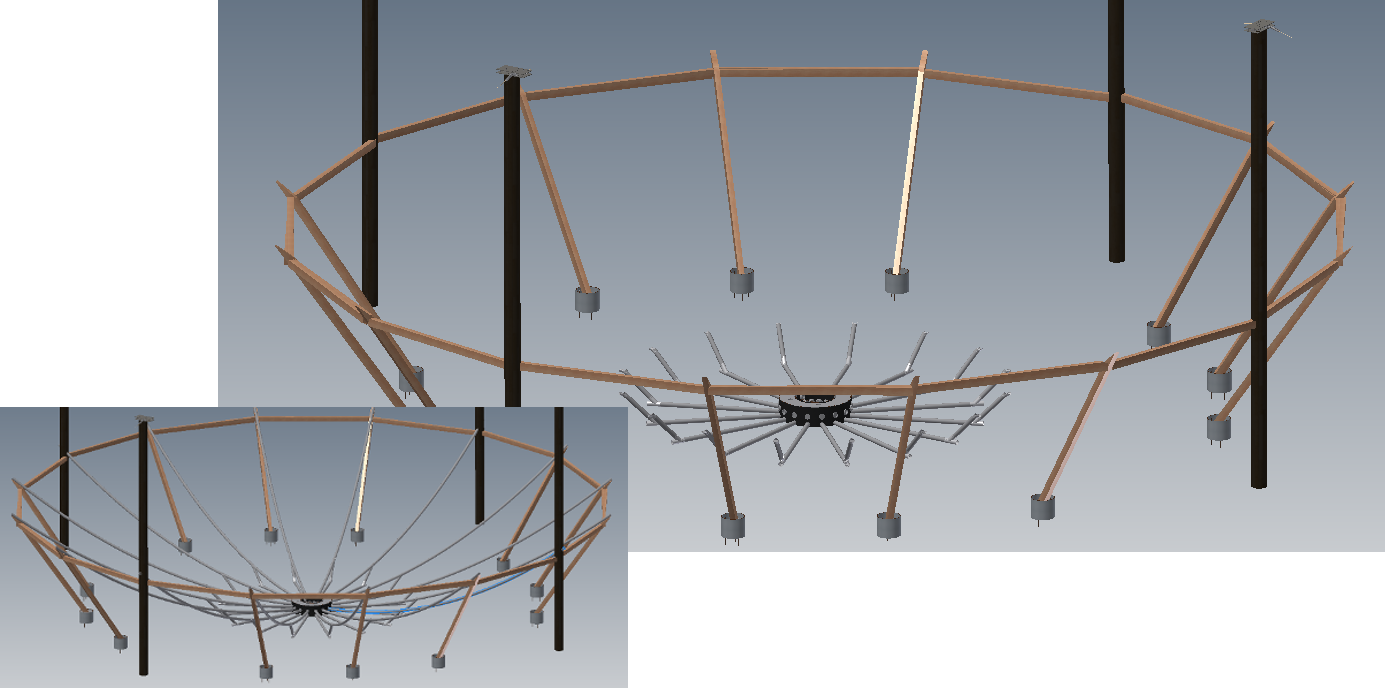
\includegraphics[width=\textwidth]{support.png}
\caption{The support system, showing the poles,stand and inner ring (held from the hub).  The inset on the lower right shows the spars.}
\label{fig:support}
\end{figure}

\subsubsection{Poles}
The principle spar support will be by wooden poles at quadrants.  These poles will also support the feed and the shield.  The posts are a key cost parameter, as 1204 are needed and they must be mechanically secure.  This is a key issue with the regular grid as they are shared (which allows for counter-tensioning as well), however outliers using their own poles and guy-lines (as will also be needed at the edges of the grid) are certainly possible.   Poles for rural single-wire earth return power distribution systems are very appropriate for this.

Adjustment mechanisms for both height and position from nominal installed positions have been designed.  The adjustment in position from expected installation accuracy is handled by the pole-top mechanism described below.  Height is handled by installing over-tall poles and trimming with a jig and laser level.  The installation accuracy should be $\pm$10cm at the pole-top.  Note that a $1^o$ tilt is about a 6cm displacement at 3.6 meters.

\subsubsection{Stands and Circumferential Support}
Between the poles will be 3 wood or metal (shown as wood) stands which will support the spar ends and the circumferential support.  The top will the cut at the proper angle to hold the end of the spar in the correct orientation.  The height and position is transferred from the poles via the circumferential supports, which also hold the top edge of the surface screen.

\subsubsection{Inner Ring}
The inner ring is made of PVC held off of the hub.  It can be made with stock PVC couplings and hold the spars at the proper angle at a given distance.  If needed, another intermediate ring can be held off of the inner ring support.

\subsection{Surface}
The surface will be the same as for PAPER ($^1/_4$\inch{} wire cloth) cut in the shape of overlapping faceted panels at each spar.  The panel will be secured by clips over the spars.  For 6\foot{} wide wire cloth, three panel types are needed per spar, for a total of 48 panels.  One lower panel will be releasable so that a person can get through to service the feed.   The total surface area is about 0.09 km$^2$.

\subsection{Splash Cone}
As discussed above, getting the ripple below about 60 dB is a key design parameter, so scattering/absorbing cones (''splash cones'') will be installed at the vertex, as well as on the bottom area of the feed.

The splash cone at the vertex will be a truncated conical pyramid with an absorbing cap.  The cone will be made of the same wire cloth as the surface and the absorbing cap will protrude from the end.  The cap can be made of standard eccosorb pyramids (with a weather cover) or using flat ferrite tiles glued onto a foam.  It will be slotted on one side to remove from around the central kevlar line.  Figure \ref{fig:hubwithsplash} shows the hub with an idealized splash cone.
\begin{figure}[H]
\centering
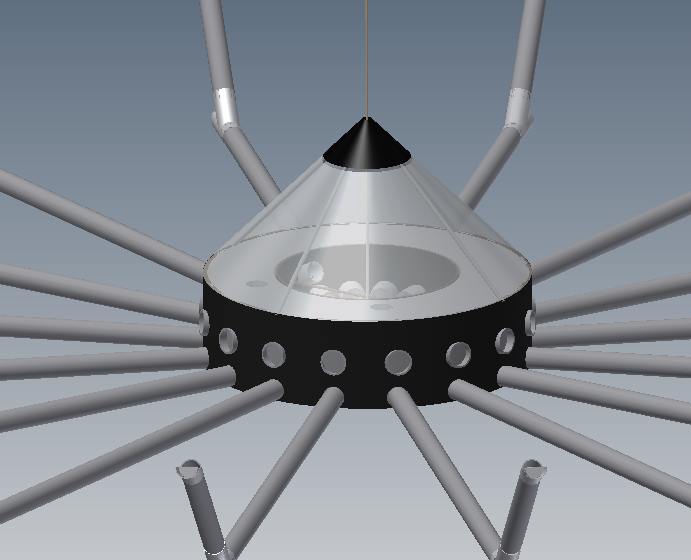
\includegraphics[width=8cm]{hubwithsplash.png}
\caption{Hub (with inner ring supports) including the idealized splash cone.}
\label{fig:hubwithsplash}
\end{figure}

At the feed, a circular ferrite tile will be glued to the feed disk.

Different arrangements at both the vertex and feed will be tested.  Cost is the main driver, as good quality absorber is expensive.

\subsection{Pole-top Assembly}
The pole-top assembly is a key mechanical interface to accurately position and tension the feed via Kevlar line.  It has to (a) handle up to $\pm$10cm positional uncertainty (b) allow tensioning of the feed support lines, and (c) be cheap.  The design incorporates two plates with ample boltholes to center a fixed point on one side, a moveable pulley to center the line going the opposite direction, and a sprocket reel to tension the line.  Note that a complete come-along incorporating the entire reel and wire rope etc. etc. costs about \$40.  Figure \ref{fig:poletop} shows engineering drawings, modulo the details of the actual reel shape.

\begin{figure}[H]
\centering
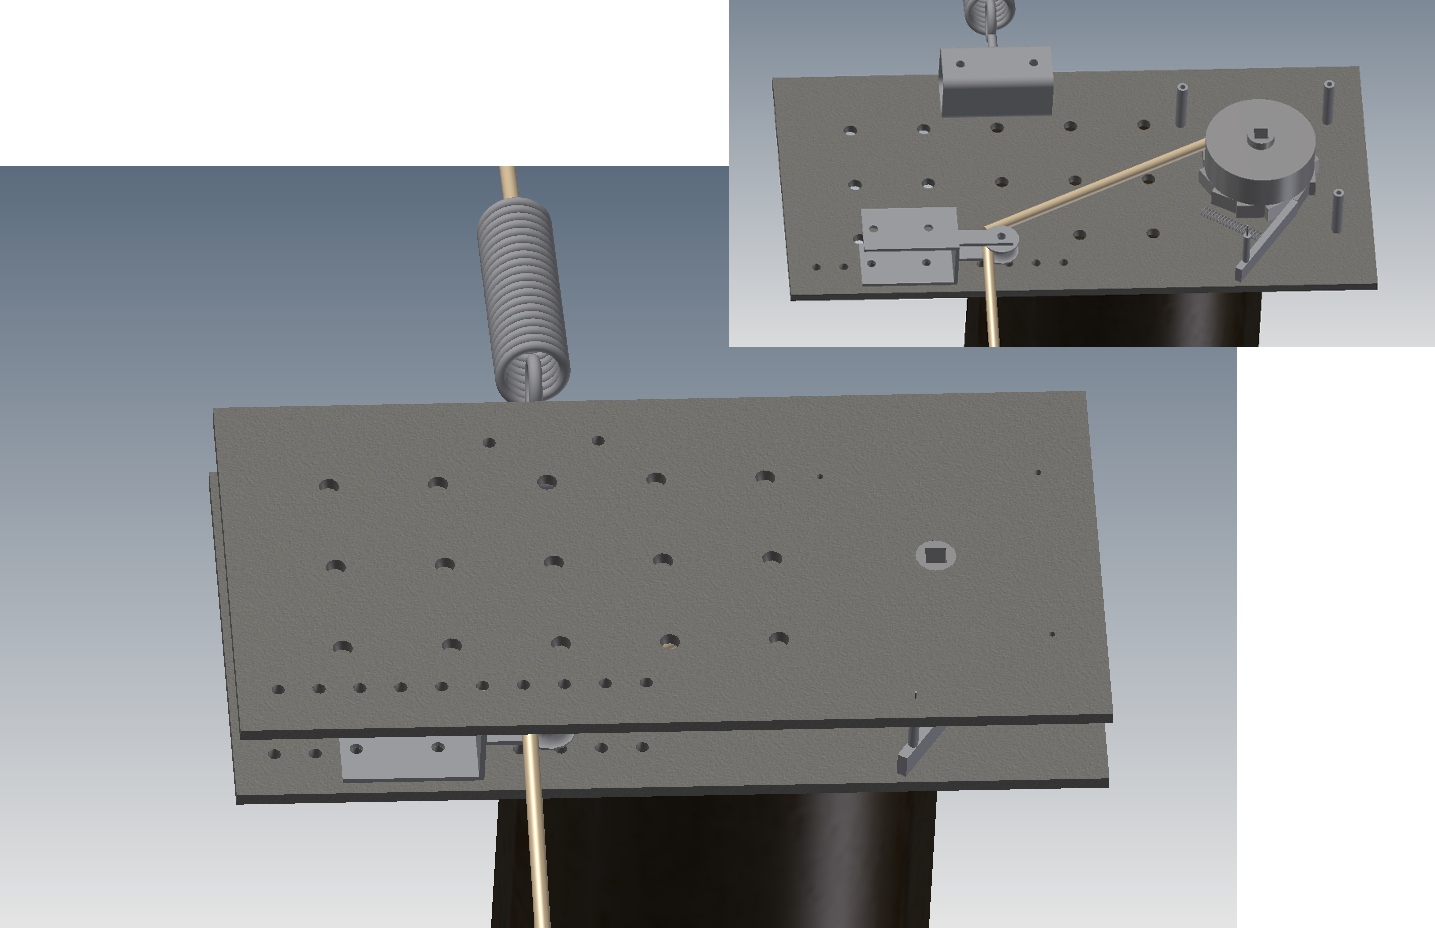
\includegraphics[width=\textwidth]{poletop.png}
\caption{Pole-top assembly with and without the top plate.}
\label{fig:poletop}
\end{figure}

\subsection{Shield}
The shield will be made of chicken wire (?) and will be strung between the poles as an “egg-crate” structure.  One direction can be contiguous while the other will intersect and will need to connect and project through.

Alternatively, if desired, the shield can be projected up from the circumference of the antenna.

\section{Front-end}
The front-end is currently based on the PAPER dipole, but held ''upside-down''.  It is supported between the poles by Kevlar line (Fig. \ref{fig:frontend}).  A central line feeding through the feed and mast between the hub and back-screen holds the feed in tension at the correct height.  The crossing Kevlar lines from the poles are at a downward angle of about 20 $^o$ and (although not as shown) each are one line to allow for centering.  The tensioning is supported by a small inner frame, from which the feed, the back-screen and central tensioning line are supported.  It also allows for some leveling of the feed, as the poles may be at slightly different heights.   A strong spring (shown in \ref{fig:poletop}) will be used to retain tension under creep.

\begin{figure}[H]
\centering
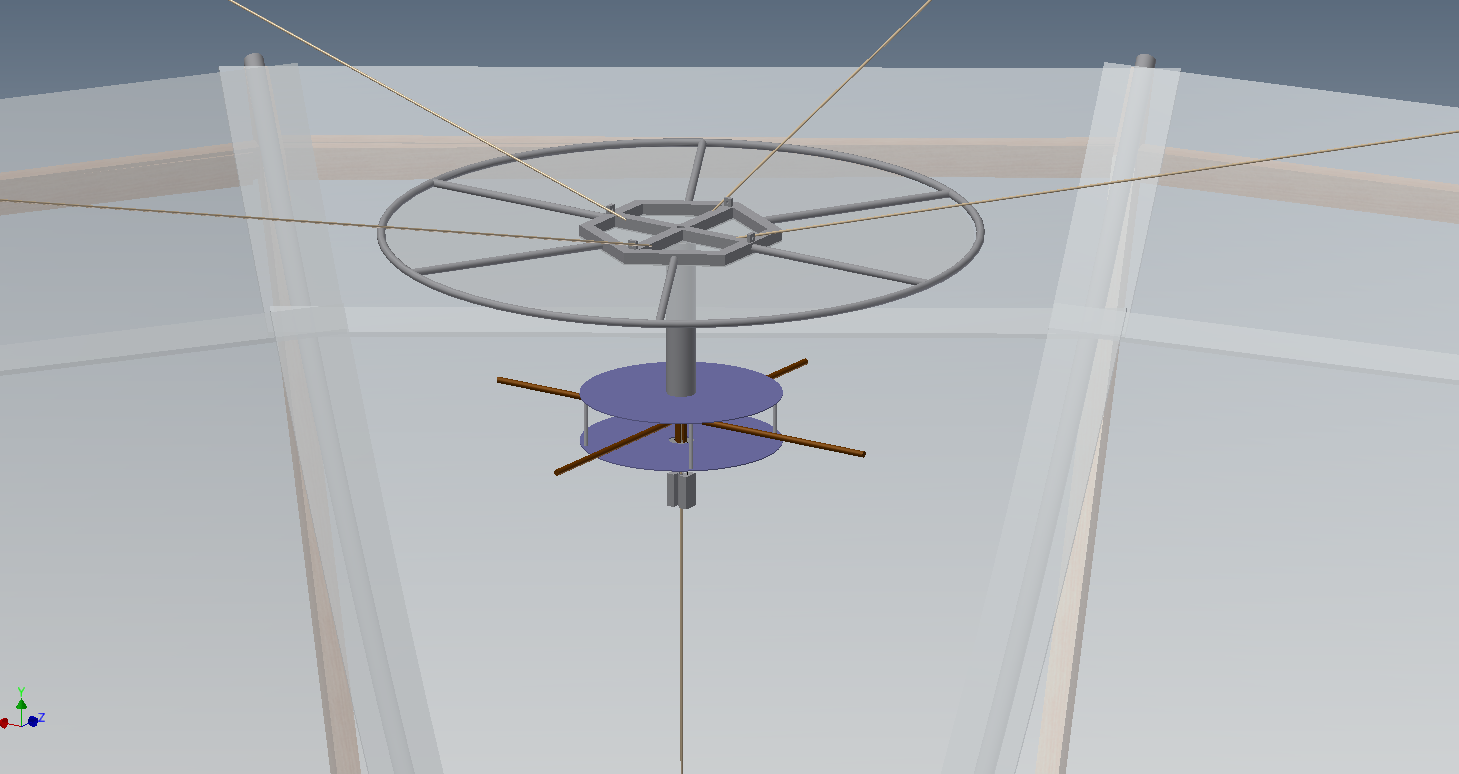
\includegraphics[width=\textwidth]{frontend.png}
\caption{Feed supported off poles with central tensioning line.}
\label{fig:frontend}
\end{figure}

The balun/low-noise amplifiers sit immediately below the feed supported off the central tensioning line.  The 50 $\Omega$ output coax follows the line down, through the hub and off to the node.  Each antenna will have the same fixed length of about 30m.

The front-end electronics may easily cover any range between 30-300 MHz.  The feed itself is roughly an octave, which may be re-centered from the nominal 150 MHz.   Extending the range adds risk associated with the actual performance (i.e., not just cost), however studies are underway on this.  The cost of increasing the bandwidth is discussed below, as it relates to the digitizer and signal transport.

\section{Node}
The node receives signals from 16 antennas (32 inputs), digitizes, does some degree of processing/packetizing and sends it down optical fiber to the correlator.  The specific architecture of the node is the critical determinant of the array flexibility.  For the strawman here (0-250 MHz), the existing design of the PAPER 16-input ADC card can be used, but joined with a Kintex FPGA to process and put onto optical fiber.   This board is currently being designed by NRAO and Berkeley and the schematic is shown in Figure \ref{fig:herald}.  More information may be found at https://casper.berkeley.edu/wiki/DAB-HERALD.

The node will accept 230VAC/50Hz single phase.  This powers the refrigerator (a stable temperature around 75$^o$F will be used), the lna's via two wires to each antenna for 12 VDC, the receivers, digitizers and data transmission.

\begin{figure}[H]
\centering
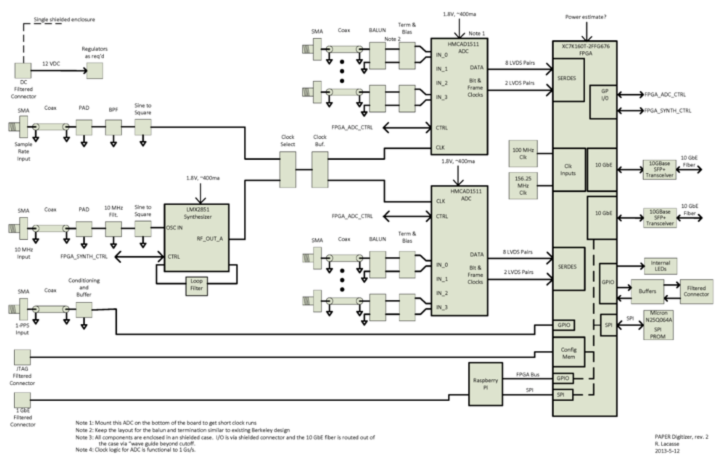
\includegraphics[width=\textwidth]{herald.png}
\caption{Schematic of the digitizer board under development.}
\label{fig:herald}
\end{figure}

\subsection{Receiver}
The analog receiver input is 50 $\Omega$ coax and, as with the front-end, may fairly easily handle 30-300 MHz.  An excellent input match is needed to keep the reflections below the level of confusion for the EOR signal.  The PAPER receiver may be used upon changing the input impedance from 75 $\Omega$ to 50 $\Omega$.

\subsection{Digitizer}
The digitizer board integrates Hittite ADCs
such as those used on CASPER's ADCx16 board with a small Kintex7 FPGA
that will be responsible for processing and formatting data into 10 GbE packets to be output
over an SFP+ connector.  This board will also implement the F-engine portion of the correlator and truncate to fewer bits (4b+4b real/imaginary) for transmitting back to the central correlator.

\section{Correlator}
The digital system that comprises a large switch and GPUs.  It should sit within the Karoo Array Processing
Building.  Note that this will likely be farther than the 1 km limit of the
node optical links, so an additional level of aggregation and long-haul
capability will likely be needed.

GPUs will serve as X-engines in the correlator (and will also be used to compress data, as discussed 
in \S\ref{sec:procData}). For HERA, we anticipate 2 Moore's Law doublings from currently deployed PAPER
technology (the Kepler 690 dual GPU card), allowing a 576-element full-Stokes correlator to be implemented with
74 GPU boxes, each containing 1 CPU, 2 dual-GPUs, and 1 dual 10GbE NIC.
If full Stokes is not needed (i.e. no U,V), the GPU system may possibly be reduced by a factor of 2.


\section{Processing and Data Management}
\label{sec:procData}
Given the sheer volume of data output from the correlator, a near-real-time processing system must
be in place to reduce data to a manageable volume.  A data compression scheme tailored to low-frequency
transit telescopes is described in Appendix A of \citet{parsons_et_al2013}.
As demonstrated on PAPER, this delay/fringe-rate compression scheme is nearly lossless from
the point of view of EoR emission locked to the celestial sphere.  Applying the full compression assuming
a maximum baseline length of 300m results in a 20x data reduction factor.  This reduces the data volume
from a campaign (180 days) to 174 TB.

\section{Reticulation}
Signal and power reticulation have been discussed above and are shown in Figure \ref{fig:heraconfig576}.  Figure \ref{fig:heraconfig576ret} below shows just the reticulation.

\subsection{Signal}
The signal path consists of a ~30m section of coaxial cable from the LNA to digitizer (same for every antenna - shown in red in Fig. \ref{fig:heraconfig576ret}), then multiplexed as 10GbE onto fiber for transmission back to the processor, as discussed above.  The processor will be in the Karoo Array Processing Building (KAPB), about 10 km distant. These cables are above ground, as currently done for PAPER.  Trenching for cables commences at the nodes and the power and fiber are run together.  Trenches from four nodes aggregate, which then further aggregrate along trench lines to the exterior of the array and onto the KAPB.

\begin{figure}[H]
\centering
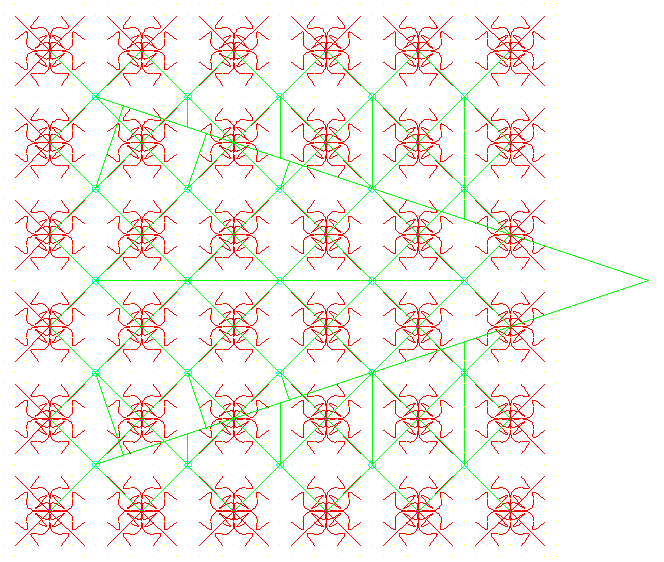
\includegraphics[width=14cm]{heraconfig576ret.png}
\caption{Drawing of signal and power reticulation.  Analog is shown in red, then the common trenching of signal and power is shown in green.  The four-node aggregate point splits the phases to those nodes.}
\label{fig:heraconfig576ret}
\end{figure}

\subsection{Power}
Power is distributed to the array via the "standard" (3.3kV) voltage.   The voltage is stepped down to and distributed as 400 VAC/3$\Phi$.  Three-phase power is distributed to four-node aggregate points, and single phase sent to the individual nodes.  The phase getting the "extra" node is cycled among the three-phases such that the overall power for the array is balanced.

\subsection{Control}
Control of the array naturally splits to three types:
\begin{enumerate}
\item Temperature:  operationally this is the most important as the concurrent temperature is used to calibrate the data, as well as set the node setpoint.  Excessive temperature is also one of the best indicators of current or future failures.  Eash node with have an external and internal temperature sensor that will send data back over the spare channel.
\item Node communication:  the node will be addressable over the spare channel with some other monitoring of node health, as well as handling any additional moves via the FPGA.
\item Correlator:  the correlator in the KAPB is fully networked and accessible for monitor and control.
\end{enumerate}

\section{Infrastructure}
The proposed site is an RF quiet site with adequate power, networking and physical area.

\bibliographystyle{plainnat}
\bibliography{/Users/ddeboer/Documents/Papers/mybibdesk}
\end{document}

